\documentclass{article}

\usepackage{amsmath}
\usepackage{graphicx}

\addtolength{\oddsidemargin}{-.3in}
\addtolength{\evensidemargin}{-.3in}
\addtolength{\textwidth}{0.6in}

\begin{document}

\title{Homework 4\\
       N-body Assembly Line}
\author{Geoffrey Ulman\\
        CSI702}
\date{March 2010}
\maketitle

\section{Design}
My parallel N-body gravitational potential code uses the assembly line programming paradigm. Each node calculates the gravitational potential for \( \frac{n}{m} \) particles where \( n \) is the number of particles and \( m \) m is the number of nodes. These will be referred to as \emph{host particles}. In addition to the \( \frac{n}{m} \) host particles, each node has \( \frac{n}{m} \) \emph{guest particles}. The algorithm has \( n \) iterations.
During each iteration, the node calculates the gravitational potential between its host particles and guest particles then passes its guest particles to one of its neighbors while receiving another set of guest particles from its other neighbor. After each node has had the particles from all other nodes as guest particles, it reports its gravitational potential values back to node 0.

\section{Challenges}
The most challenging portion of the parallel MPI implementation of the code was handling the particle data files. I encountered difficulties because I forgot that the nodes on the cds cluster use shared storage, so there was actually no need to copy data files to particular nodes. The slight differences between the output of the parallel and serial codes also caused me to spend significant effort debugging the parallel code (see the Section \ref{outputcomp} for details).

\section{MPI Commands}
Like all MPI programs, the commands \verb!MPI_Init!, \verb!MPI_Comm_size!, \verb!MPI_Comm_rank!, and \verb!MPI_Finalize! were used to initialize and get basic information about the MPI environment. Because data was being passed in a ring, \verb!MPI_Cart_create! was used to create a new Cartesian comm group and \verb!MPI_Cart_shift! was used to determine the coordinates of the nodes neighbors. In addition, \verb!MPI_Cart_coords! was used to determine whether the node was in an even or odd position in the new Cartesian comm group. Data was sent using \verb!MPI_Isend! and \verb!MPI_Irecv! so that processing of the last group of host particles could be performed while the new group of host particles was being received. Finally, completion of the communications in each iteration was checked with \verb!MPI_Waitall!.

\section{Performance Analysis}
Figure \ref{chart1} compares the parallel and serial codes for varying particle counts. For instances of the problem smaller than approximately 5000 particles, the overhead of setting up and performing communications between nodes actually overwhelms the advantages of parallel computation and the serial code runs faster. In circumstances where many independent small problems had to be computed, the serial approach might be superior. However, with more than 5000 particles, the \(n^2\) nature of the problem becomes very apparent in the serial code timing results.

\begin{figure}
\centering
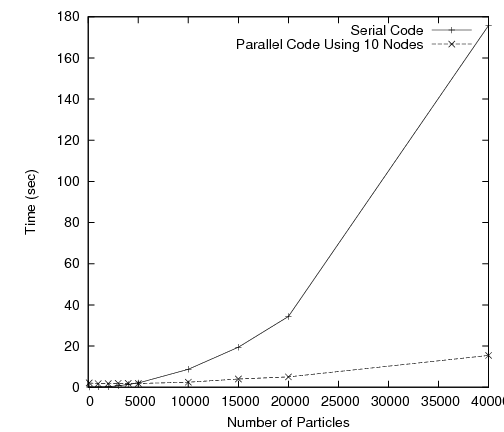
\includegraphics[width=0.6\textwidth]{img/timing_data_variable_particles.png}
\caption{Parallel and Serial Timing Results for Variable Particle Count}
\label{chart1}
\end{figure}

It is also interesting to explore the effect of varying the number of nodes used in the parallel code. This analysis was performed for both 10,000 particles and 100,000 particles with 2 through 1000 nodes. Figure \ref{chart2} indicates that the best time in the 10,000 particle case occurred for 10 nodes with 1000 particles each. The best time in the 100,000 particle case occurred at 100 nodes, which also corresponded to 1000 particles per node (although the timing results were very similar for 10 through 200 nodes).

Because the parallel code was run on a cluster of 10 nodes, the decreased performance for less than 10 nodes is simply due to the cluster not being fully utilized. However, as the number of nodes gets very large, performance again decreases. This could be due to a number of factors. Overhead due to context switches between the large number of processes on each node may have hindered performance. Also, as the number of particles per node decreases, there is less computation to hide the communication latency. With too many nodes, processors must sit idle after they have finished computation on the current batch of guest particles while they wait for the next batch to arrive.

\begin{figure}
\centering
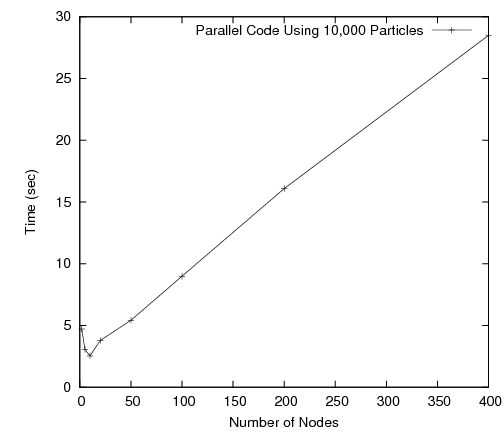
\includegraphics[width=0.6\textwidth]{img/timing_data_10000_particles.png}
\caption{Parallel and Serial Timing Results for 10,000 Particles}
\label{chart2}
\end{figure}

\begin{figure}
\centering
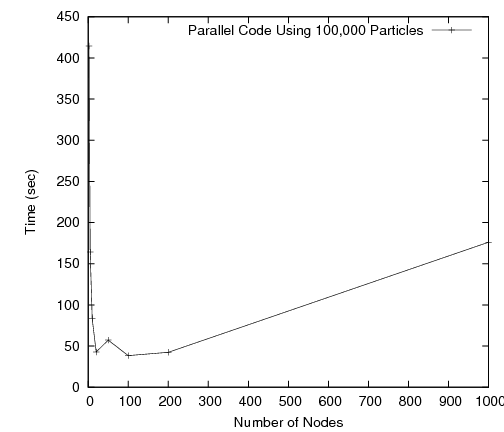
\includegraphics[width=0.6\textwidth]{img/timing_data_100000_particles.png}
\caption{Parallel and Serial Timing Results for 100,000 Particles}
\label{chart3}
\end{figure}

Although the parallel code is significantly faster for large data sets, the code is approximately 4 times longer than the serial code. The serial code essentially directly implements the mathematics, making its purpose immediately clear to a reader. The parallel code, on the other hand, obscures the core mathematics behind the communications. Because the algorithm must be modified to take advantage of the particular communication pattern and realities of communication latency, the purpose of the code is less immediately clear.

\section{Output Comparison}
\label{outputcomp}
My first version of the code used the \verb!MPI_FLOAT! data type to transfer data between nodes the and c \verb!float! to store data on the nodes. However, for large computations the output of the serial and parallel codes were extremely close but not identical. I was not able to determine the cause, but I believe error was introduced in translating between c \verb!float! and \verb!MPI_FLOAT!. When I modified the code to work with c \verb!double! and \verb!MPI_DOUBLE! the calculated potentials were identical between the parallel and serial codes to the precision recorded.

\begin{thebibliography}{9}

\bibitem{cpl}
  Brian W. Kernighan and Dennis M. Ritchie,
  \emph{The C Programming Language},
  Prentice Hall PTR, New Jersey,
  2009.

\end{thebibliography}

\end{document}
